\documentclass[8pt,dvipsnames]{beamer}
\usepackage[T1]{fontenc}
\usepackage{libertinus}
\usepackage{amsmath}
\usepackage[most]{tcolorbox}
\usepackage{graphicx}

\usepackage{hyperref}
%python 
\usepackage{listings}
% Default fixed font does not support bold face
\DeclareFixedFont{\ttb}{T1}{txtt}{bx}{n}{8} % for bold
\DeclareFixedFont{\ttm}{T1}{txtt}{m}{n}{8}  % for normal

% Custom colors
\usepackage{color}
\definecolor{deepblue}{rgb}{0,0,0.5}
\definecolor{deepred}{rgb}{0.6,0,0}
\definecolor{deepgreen}{rgb}{0,0.5,0}

\usepackage{listings}

% Python style for highlighting
\newcommand\pythonstyle{\lstset{
		language=Python,
		basicstyle=\ttm,
		morekeywords={self},              % Add keywords here
		keywordstyle=\ttb\color{deepblue},
		emph={MyClass,__init__},          % Custom highlighting
		emphstyle=\ttb\color{deepred},    % Custom highlighting style
		stringstyle=\color{deepgreen},
		frame=tb,                         % Any extra options here
		showstringspaces=false
}}


% Python environment
\lstnewenvironment{python}[1][]
{
	\pythonstyle
	\lstset{#1}
}
{}

% Python for external files
\newcommand\pythonexternal[2][]{{
		\pythonstyle
		\lstinputlisting[#1]{#2}}}

% Python for inline
\newcommand\pythoninline[1]{{\pythonstyle\lstinline!#1!}}

\usepackage{xcolor}  
\newcommand{\cb}[1]{{\color{CadetBlue}#1}}

\usepackage{pgfplots}
\pgfplotsset{compat=newest}
\setlength{\parskip}{0.5em}

\usepackage{setspace}
\setstretch{1.25}  
\usetheme{Singapore}
\setbeamertemplate{navigation symbols}{}

\setbeamertemplate{footline}{
    \leavevmode%
    \hbox{%
        \begin{beamercolorbox}[wd=.5\paperwidth,ht=2.25ex,dp=1ex,center]{author in head/foot}%
            % Customize this part if you want to add author or date information
        \end{beamercolorbox}%
        \begin{beamercolorbox}[wd=.5\paperwidth,ht=2.25ex,dp=1ex,right]{title in head/foot}%
            \usebeamerfont{title in head/foot}\insertframenumber{} / \inserttotalframenumber\hspace*{2ex} 
        \end{beamercolorbox}}%
    \vskip0pt%
}

\title{CSE574 Introduction to Machine Learning}
\subtitle{Dimensionality Reduction}
\author{Jue Guo}
\institute{University at Buffalo}
\date{\today}

\begin{document}
\begin{frame}
    \titlepage
\end{frame}
\begin{frame}
    \frametitle{Outline}
    \tableofcontents
\end{frame}

\section{Feature Selection}
\begin{frame}
    \frametitle{Feature Selection}
    \begin{itemize}
        \item Compare and contrast the difference techniques used for dimensionality reduction.
        \item Use the appropriate statistical test when performing filter-based feature selection techniques.
        \item Describe the steps in recursive feature elimination.
        \item Describe the steps in forward and backward sequential feature selection.
        \item Explain the advantages of using embedded methods over filter-based and wrapper techniques.
    \end{itemize}
\end{frame}

\subsection{Dimensionality Reduction}
\begin{frame}
    \frametitle{Dimensionality Reduction}
    \textbf{Dimensionality Reduction} is the process of reducing the number of features in a dataset while preserving as much of the information as possible.
    \begin{itemize}
        \item The number of features can be reduced by combining feature to create new features in a process called \textit{feature extraction} or selecting a subset of features in a process called \textit{feature selection}.
        \item The primary goal is to simplify the data representation and make data more manageable and interpretable.
    \end{itemize}
    Dimensionality reduction also reduces computation cost, which is very important when working with certain machine learning algorithms.
\end{frame}

\begin{frame}
    \frametitle{Dimensionality Reduction}
    \begin{figure}[ht]
        \centering
        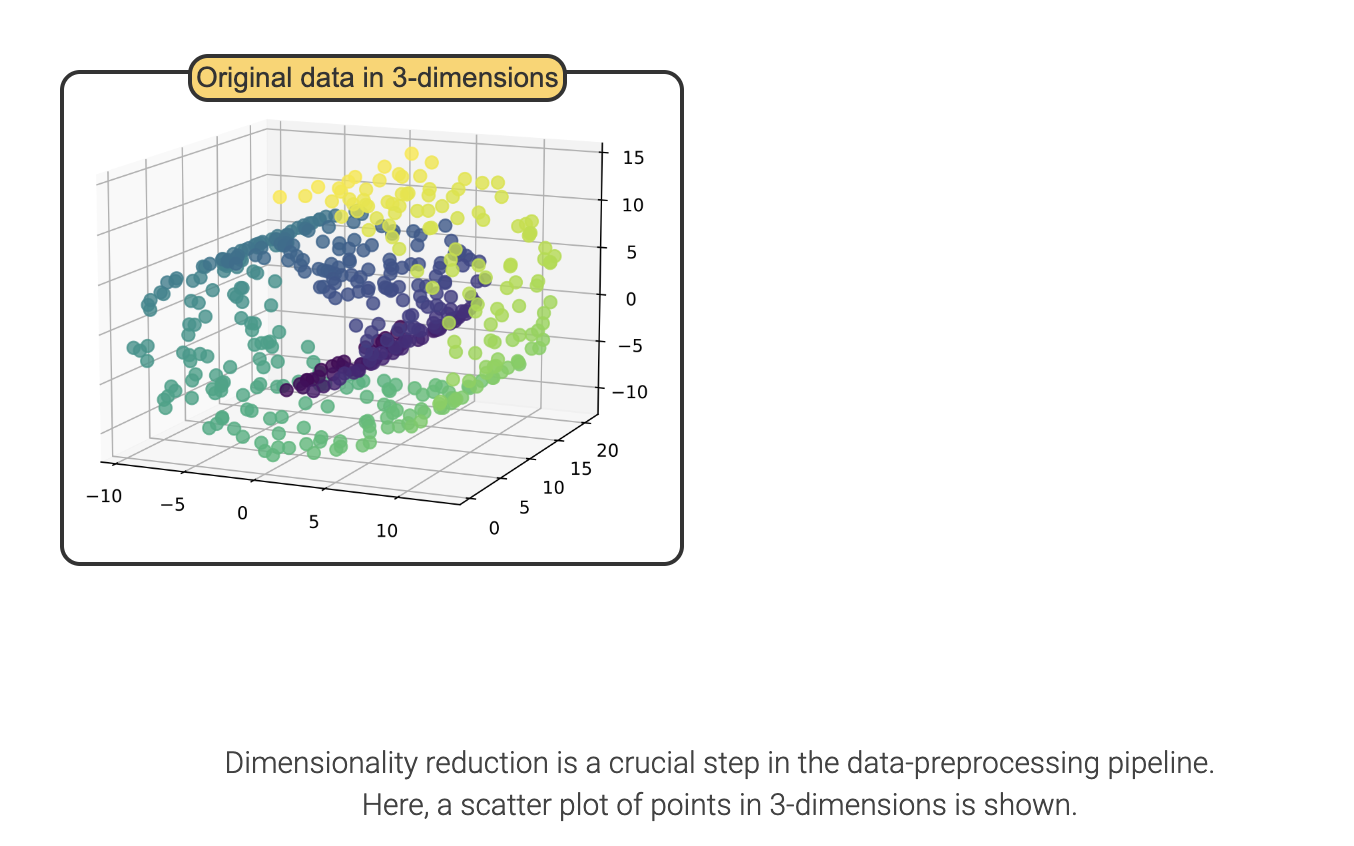
\includegraphics[width=0.8\textwidth]{imgs/DR_1.png}
    \end{figure}
\end{frame}

\begin{frame}
    \frametitle{Dimensionality Reduction}
    \begin{figure}[ht]
        \centering
        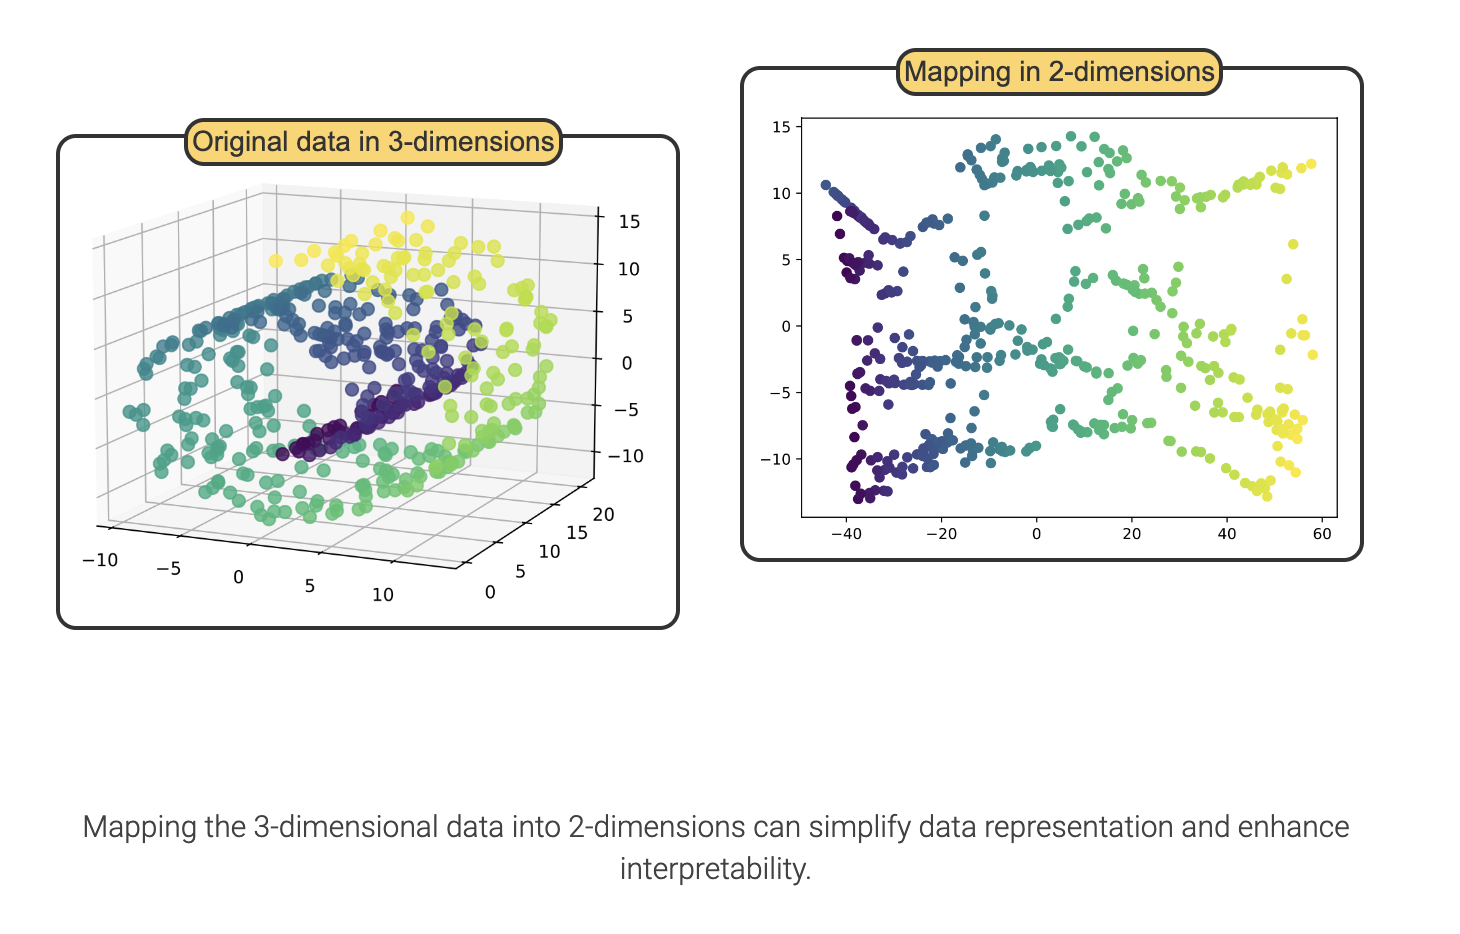
\includegraphics[width=0.8\textwidth]{imgs/DR_2.png}
    \end{figure}
\end{frame}

\begin{frame}
    \frametitle{Dimensionality Reduction}
    \begin{figure}[ht]
        \centering
        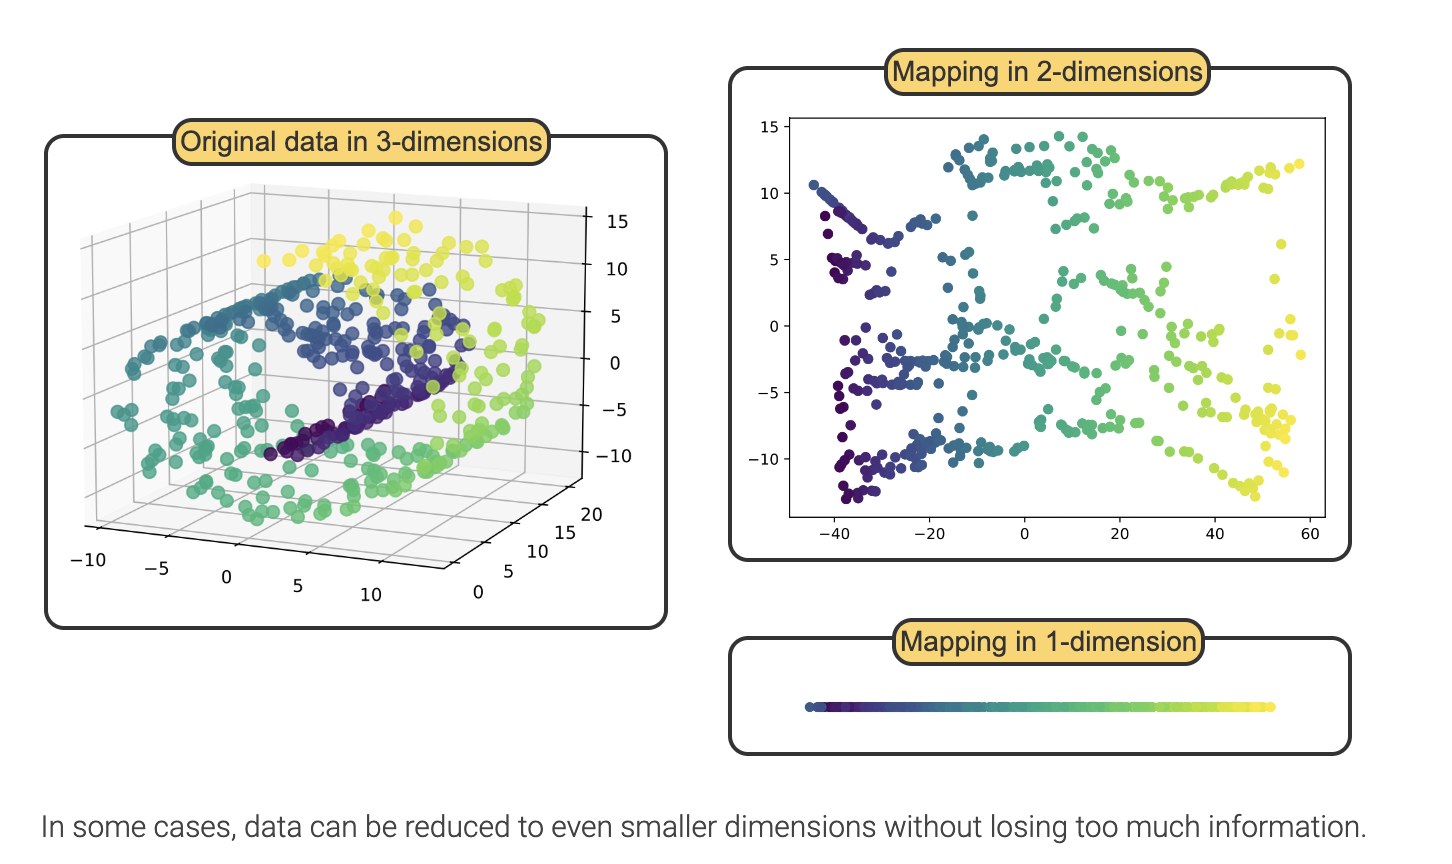
\includegraphics[width=0.8\textwidth]{imgs/DR_3.png}
    \end{figure}
\end{frame}
\subsection{Introduction to feature selection}
\begin{frame}
    \frametitle{Introduction to feature selection}
    \textbf{Feature selection} is a process of selecting a subset of features from a dataset that are most relevant for a machine learning task.
    \begin{itemize}
        \item The main goals of feature selection are to improve model performance and reduce computational complexity.
        \item Feauture selection methods can be classified into three broad categories: filter-based methods, wrapper methods and embedded methods.
    \end{itemize}
\end{frame}

\begin{frame}
    \frametitle{Introduction to feature selection}
    \begin{itemize}
        \item \textbf{Filter-based methods} rank features based on the relationship between the input and output features.
        \item \textbf{Wrapper methods} select features by iteratively building and evaluating models on a subset of features.
        \item \textbf{Embedded methods} integrate the feature selection processes into the training of a machine learning model.
    \end{itemize}
\end{frame}

\subsection{Filter-based methods}
\begin{frame}
    \frametitle{Filter-based methods}
    Filter-based methods rank the importance of each feature based on statistical tests involving a single feature. The required statistical test depends on the data type of the input and output features.
    \begin{itemize}
        \item Ex: In the Wisconsin Breast Cancer dataset, the input features are all numeric, while the output feature is categorical, so comparing the \(F\)-statistic from a logistic regression model containing a single input feature would be appropriate.
    \end{itemize}
\end{frame}

\begin{frame}
    \frametitle{Filter-based methods}
    \begin{figure}[ht]
        \centering
        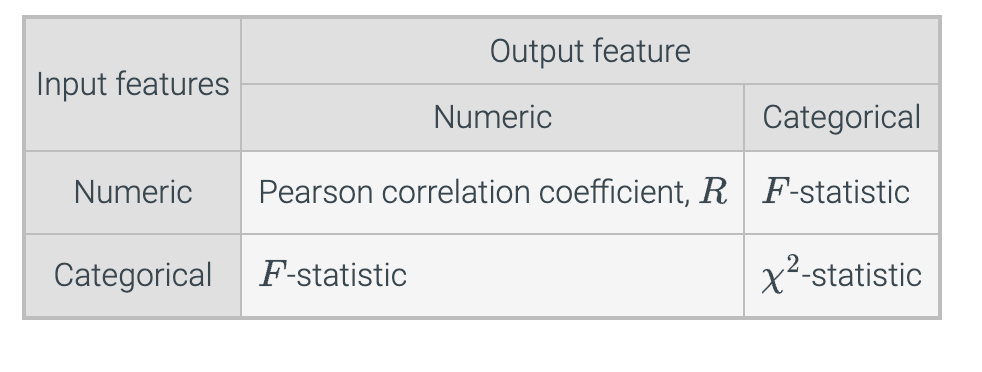
\includegraphics[width=0.8\textwidth]{imgs/DR_4.png}
    \end{figure}
\end{frame}

\subsection{Wrapper methods: Recursive feature elimination}
\begin{frame}
    \frametitle{Wrapper methods: Recursive feature elimination}
    A common wrapper method is recursive feature elimination.
    \begin{itemize}
        \item \textbf{Recursive feature elimination (RFE)} iteratively removes the least important features from the dataset until a desired number of features is reached.
        \item The RFE algorithm takes in two hyperparameters : an estimator and the desired number of features.
    \end{itemize}
    Select a machine learning model and the desired number of features.
    \begin{enumerate}
        \item Train a machine learning model using all features.
        \item Rank the importance of each feature.
        \item Eliminate the least important feature.
    \end{enumerate}
    Repeat steps 1-3 until the desired number of features remains or model performance stabilizes.
\end{frame}

\subsection{Wrapper methods: Sequential feature selection}

\begin{frame}
    \frametitle{Wrapper methods: Sequential feature selection}
    Since a dataset with p features contains \(2^{p}\) feature subsets, an exhaustive search for the best performing feature subset is often prohibitive
    for datasets with a large number of features.
    \begin{itemize}
        \item \textbf{Sequential feature selection (SFS)} selects or removes features from the dataset in a step-by-step manner by using cross validation techniques to evaluate model performance at each iteration.
    \end{itemize}
    The two main types of SFS are forward selection and backward selection. Although similar, forward and backward selection do not always result in the same model.
\end{frame}
\begin{frame}
    \frametitle{The two main types of SFS}
    \begin{itemize}
        \item \textbf{Sequential forward selection} starts with no features and iteratively adds features to the model starting with the most important feature.
        \item \textbf{Sequential backward selection} starts with all features in the dataset and iteratively removes features from the model starting with the least important feature.
    \end{itemize}
    Both forward and backward selection is monotonic, which means that features cannot be removed once added. Similarly, features cannot be added once removed.
\end{frame}

\begin{frame}
    \frametitle{Sequential Forward Selection}
    Suppose a dataset has \(p\) features. Begin with an empty feature set. For iteration \(i=1, \ldots, p\) :
    \begin{enumerate}
        \item Generate all subsets of size \(i\) that contain features from the previous iteration. \(p+1-i\) subsets are generated at step \(i\). Each
              subset will contain the chosen subset from the previous iteration and one additional feature.
        \item Evaluate model performance on each subset.
        \item Keep the added feature from the subset with the best score.
    \end{enumerate}
    Compare the performance of feature subsets for iterations \(1, \ldots, p\). The feature subset with the best evaluation score is selected. For
    ties, the feature subset with less features should be selected.
\end{frame}

\begin{frame}
    \frametitle{Sequential backward selection}
    Suppose a dataset has \(p\) features. Begin with a feature set with all \(p\) features. For iteration \(i=1, \ldots, p\) :
    \begin{enumerate}
        \item Generate all subsets of size \(p-i\) that exclude features removed from the previous iteration. \(p+1-i\) subsets are generated at
              step \(i\). Each subset will contain the chosen subset from the previous iteration with one less feature.
        \item Evaluate model performance on each subset.
        \item Remove the feature that is missing from the subset with the best score.
    \end{enumerate}
    Compare the performance of feature subsets for iterations \(1, \ldots, p\). The feature subset with the best evaluation score is selected. For
    ties, the feature subset with less features should be selected.
\end{frame}

\subsection{Embedded methods}

\begin{frame}
    \frametitle{Embedded methods}
    An embedded method for feature selection selects the most relevant features when training a machine learning model. Embedded methods differ from filter methods and wrapper methods in that feature selection is an integral part of the model building process.
    \begin{itemize}
        \item Embedded methods typically incorporate feature selection as a step within the algorithm itself or through model-specific techniques.
        \item Common examples are tree-based methods (Ex: random forest) and regularization techniques (Ex: LASSO regression).
    \end{itemize}

\end{frame}

\begin{frame}
    \frametitle{Embedded methods}
    Advantages of embedded methods include:
    \begin{itemize}
        \item Efficiency—Embedded methods are efficient, because feature selection is integrated into the training process. Feature selection is automated and does not involve a separate step.
        \item Improved interpretability of models—In some cases, embedded methods highlight which features are most influential.
        \item Flexibility in model selection—Embedded methods select the best features while simultaneously choosing an appropriate machine learning algorithm. This flexibility can be advantageous when exploring various modeling approaches.
    \end{itemize}
\end{frame}
\section{Feature extraction using linear techniques}
\begin{frame}
    \frametitle{Feature extraction using linear techniques}
    \begin{itemize}
        \item Perform factor extraction using multiple linear techniques.
        \item Select the appropriate techniques for different use cases.
        \item Identify the terminology used in principal component analysis, independent component analysis, and factor analysis and list each algorithm's steps.
    \end{itemize}
\end{frame}
\subsection{Introduction to linear feature extraction}
\begin{frame}
    \frametitle{Introduction to linear feature extraction}
    Feature extraction is the process of creating new features from raw data to reduce dimensionality and identify important patterns. Often, raw data cannot be really used for a machine learning algorithm, so data should be transformed into a format from which feature can be extracted.

    Feature extraction can lead to improved model performance, reduced training times, and better generalization to new data. \textbf{Linear feature extraction} creates new features by taking linear combinations of existing features instead of using all original features. Linear feature extraction techniques include:
    \begin{itemize}
        \item Principal component analysis
        \item Independent component analysis
        \item Factor analysis
    \end{itemize}
\end{frame}

\subsection{Principal Component Analysis(PCA)}
\begin{frame}
    \frametitle{Principal Component Analysis}
    \textbf{Principal Component Analysis}, or \textbf{PCA}, is a procedure that transforms data into a new coordinate system in which the variance of the data along each axis is maximized.
    \begin{itemize}
        \item \textbf{Principal components} are the axes used in PCA. PCA is most commonly used for image compression, noise reduction, and anomaly detection.
    \end{itemize}
    An important step in performing PCA is finding the eigendecomposition of the covariance matrix.
    \begin{itemize}
        \item  A \textbf{covariance matrix} contains the direction of the relationships between features in the dataset.
        \item \textbf{Eigendecomposition} decomposes a covariance matrix into eigenvalues and eigenvectors.
    \end{itemize}
\end{frame}

\begin{frame}
    \frametitle{Principal Component Analysis}
    This decomposition expresses a covariance matrix \(C\) as a sequence of scale and rotation transformations. Mathematically, \(C=P \Lambda P^{T}\) where \(P\) is a matrix whose columns are eigenvectors, and \(\Lambda\) is a matrix whose diagonals are eigenvalues. In the context of PCA:
    \begin{itemize}
        \item An \textbf{eigenvalue} is a scalar that indicates the amount of variance explained by the corresponding principal component.
        \item An \textbf{eigenvector} is a unit vector that describes the direction of the corresponding principal component.
    \end{itemize}
\end{frame}

\begin{frame}
    \frametitle{Algorithm: PCA}
    \begin{enumerate}
        \item \textit{Standardize the data.} Since PCA is sensitive to scale, data should be standardized to have a mean of 0 and a standard deviation of 1.
        \item \textit{Compute the covariance matrix.} The covariance between features \(X\) and \(Y\) is given by
              $$
                  \operatorname{cov}(X, Y)=\frac{\sum\left(x_{i}-\bar{x}\right)\left(y_{i}-\bar{y}\right)}{N}
              $$
              where:
              \begin{itemize}
                  \item \(x_{i}\) and \(y_{i}\) are the standardized values for the \(i\) th instance
                  \item \(\bar{x}\) and \(\bar{y}\) are the means of the standardized values
                  \item \(N\) is the number of instances
              \end{itemize}
              The covariance matrix \(C\) is a \(p \times p\) matrix where \(p\) is the number of features and the off-diagonal elements contain the covariances between two features. The diagonal elements contain the variances of each feature.
    \end{enumerate}
\end{frame}

\begin{frame}
    \frametitle{Algorithm: PCA}
    \begin{enumerate}
        \setcounter{enumi}{2}
        \item \textit{Compute the eigenvalues and corresponding eigenvectors.} The eigenvalues and eigenvectors of the covariance matrix \(C\) are
              obtained by solving the equation
              $$
                  C \mathbf{v}=\lambda \mathbf{v}
              $$
              where \(\lambda\) is an eigenvalue and \(\mathbf{v}\) is the corresponding eigenvector.
        \item \textit{Sort and select the principal components.} The principal components with the largest eigenvalues capture the most variance in the data.

              A \textbf{scree plot} can be used to choose the number of components to retain. A scree plot is a line plot of explained variance or eigenvalues of principal components. The principal components at or before the elbow or leveling off point should generally be retained.
        \item Transform the data. The projection matrix uses the eigenvectors with the highest eigenvalues as columns and transforms the original data into a lower-dimensional space. The projection is obtained using the equation
              $$
                  \text { new data }=\text { standardized data } * \text { projection matrix }
              $$
    \end{enumerate}
\end{frame}

\begin{frame}
    \frametitle{Applying PCA to the MNIST digits dataset.}
    \begin{figure}[ht]
        \centering
        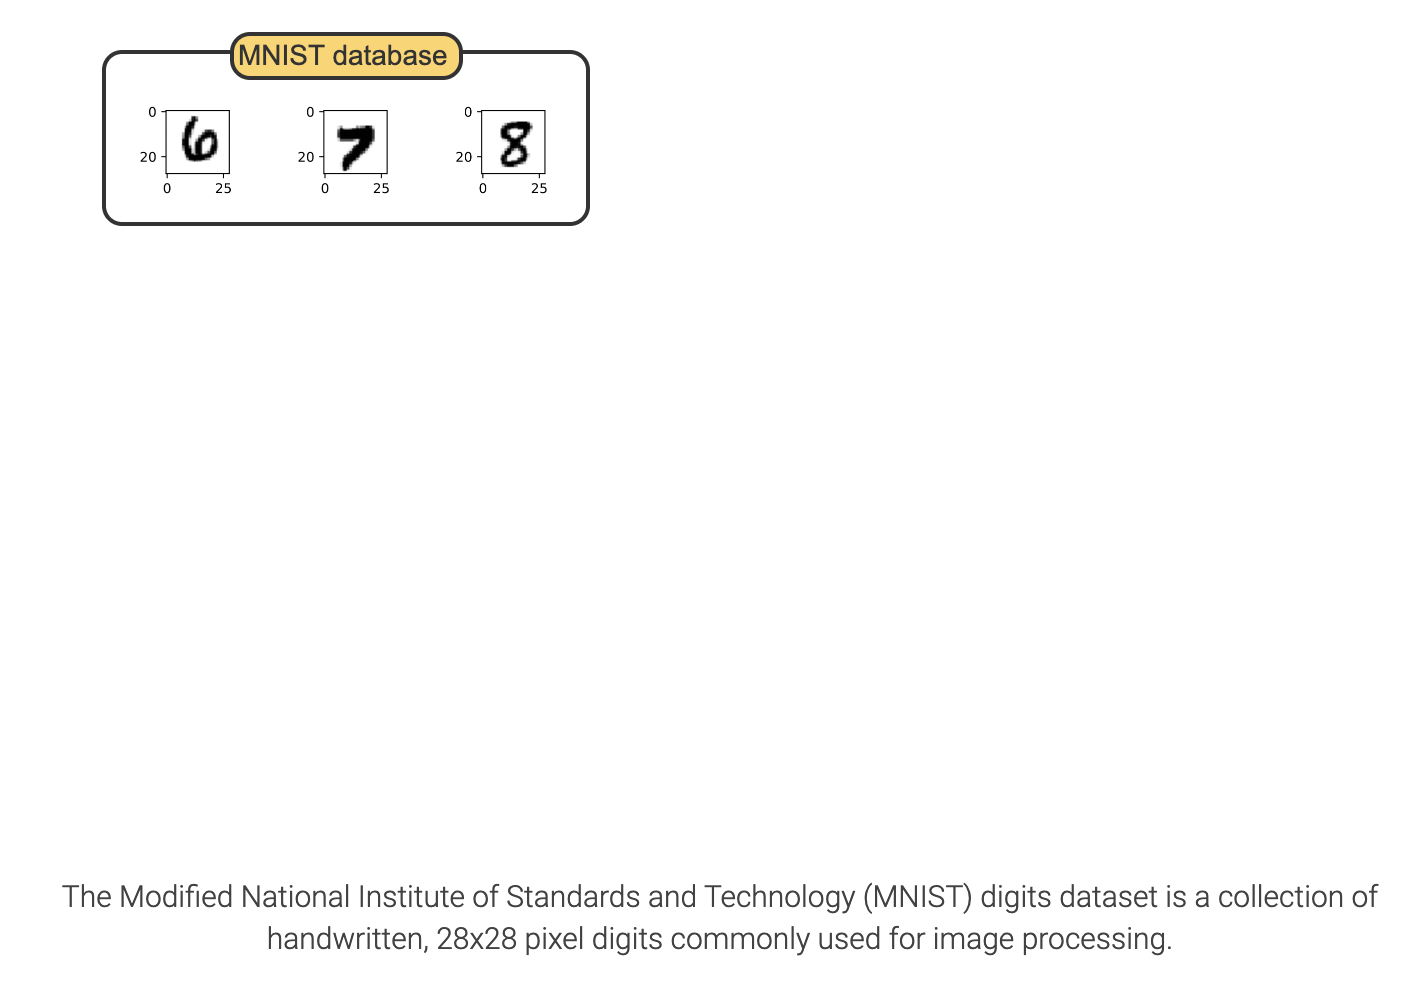
\includegraphics[width=0.8\textwidth]{imgs/DR_5.png}
    \end{figure}
\end{frame}

\begin{frame}
    \frametitle{Applying PCA to the MNIST digits dataset.}
    \begin{figure}[ht]
        \centering
        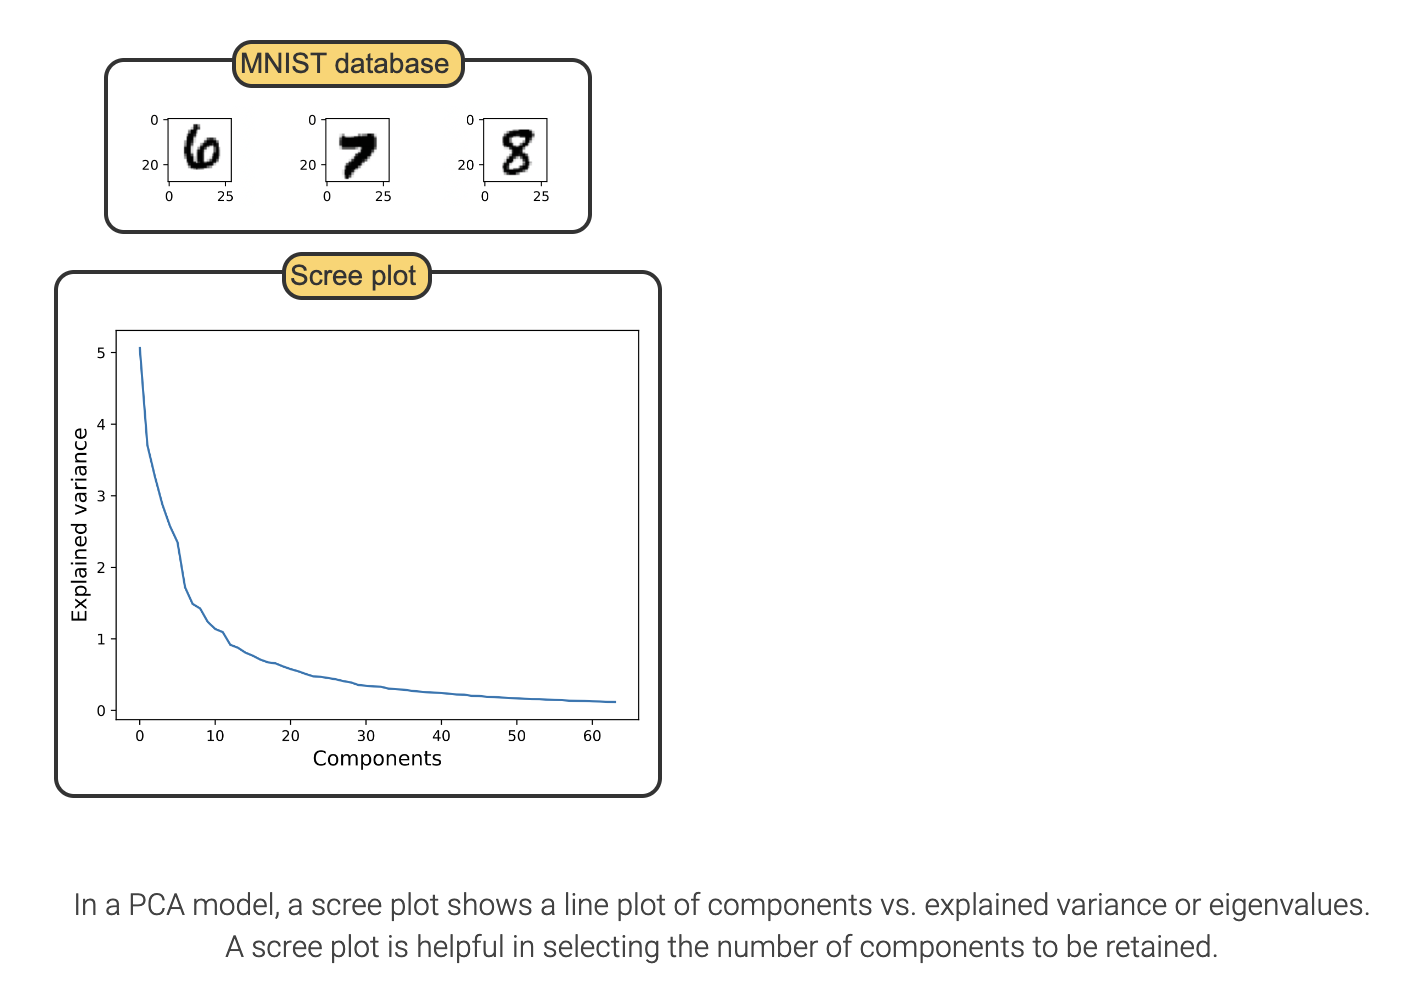
\includegraphics[width=0.8\textwidth]{imgs/DR_6.png}
    \end{figure}
\end{frame}

\begin{frame}
    \frametitle{Applying PCA to the MNIST digits dataset.}
    \begin{figure}[ht]
        \centering
        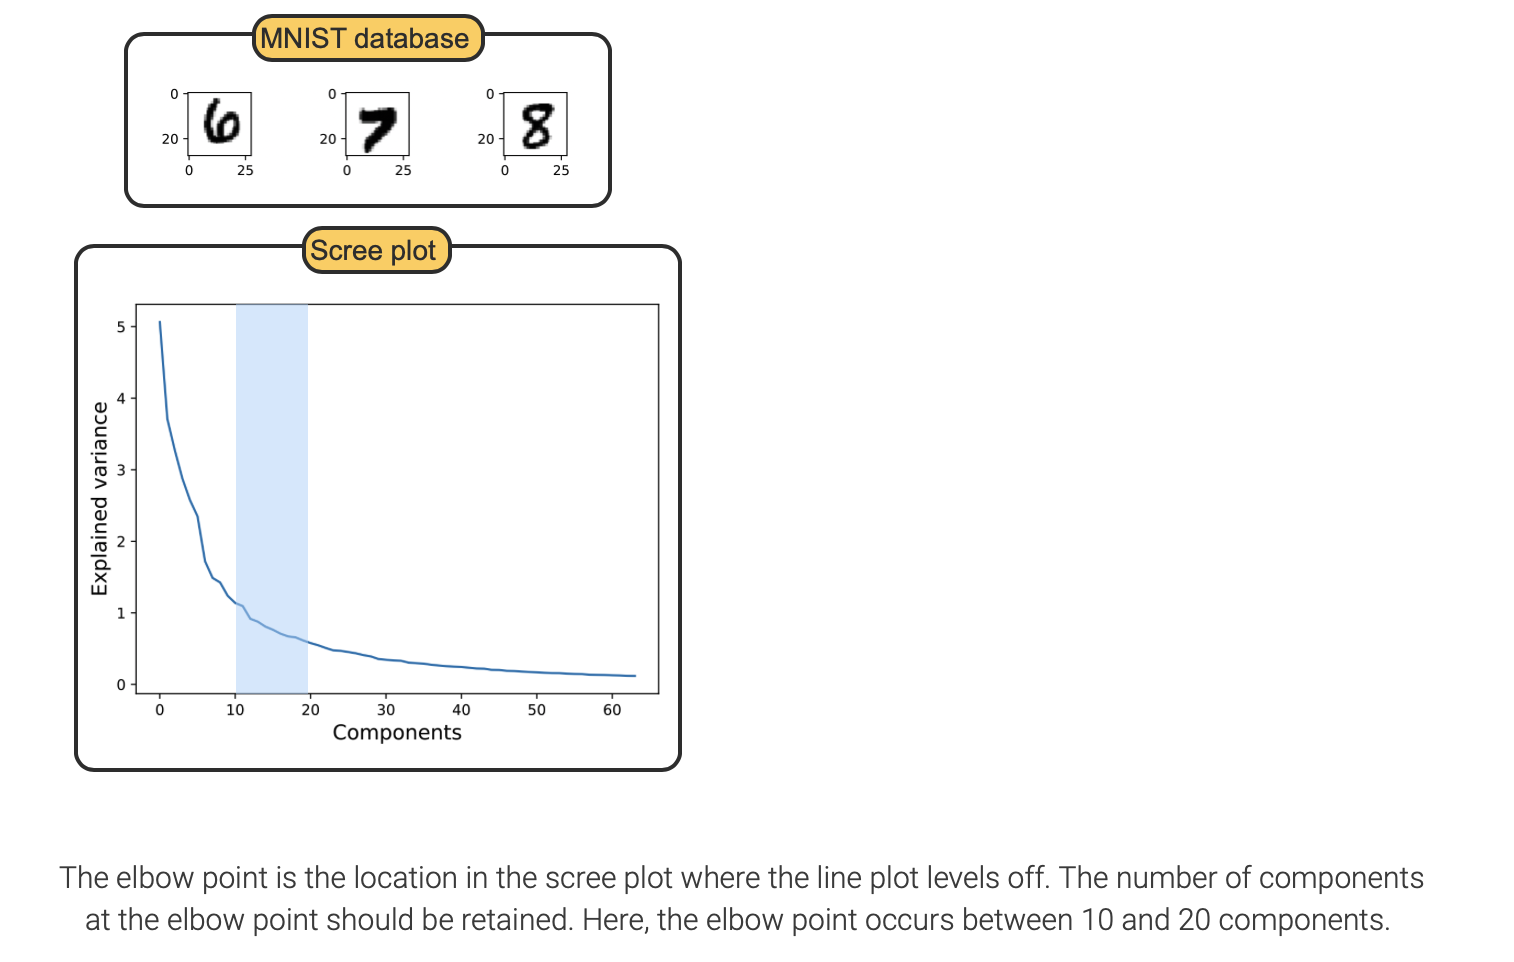
\includegraphics[width=0.8\textwidth]{imgs/DR_7.png}
    \end{figure}
\end{frame}

\begin{frame}
    \frametitle{Applying PCA to the MNIST digits dataset.}
    \begin{figure}[ht]
        \centering
        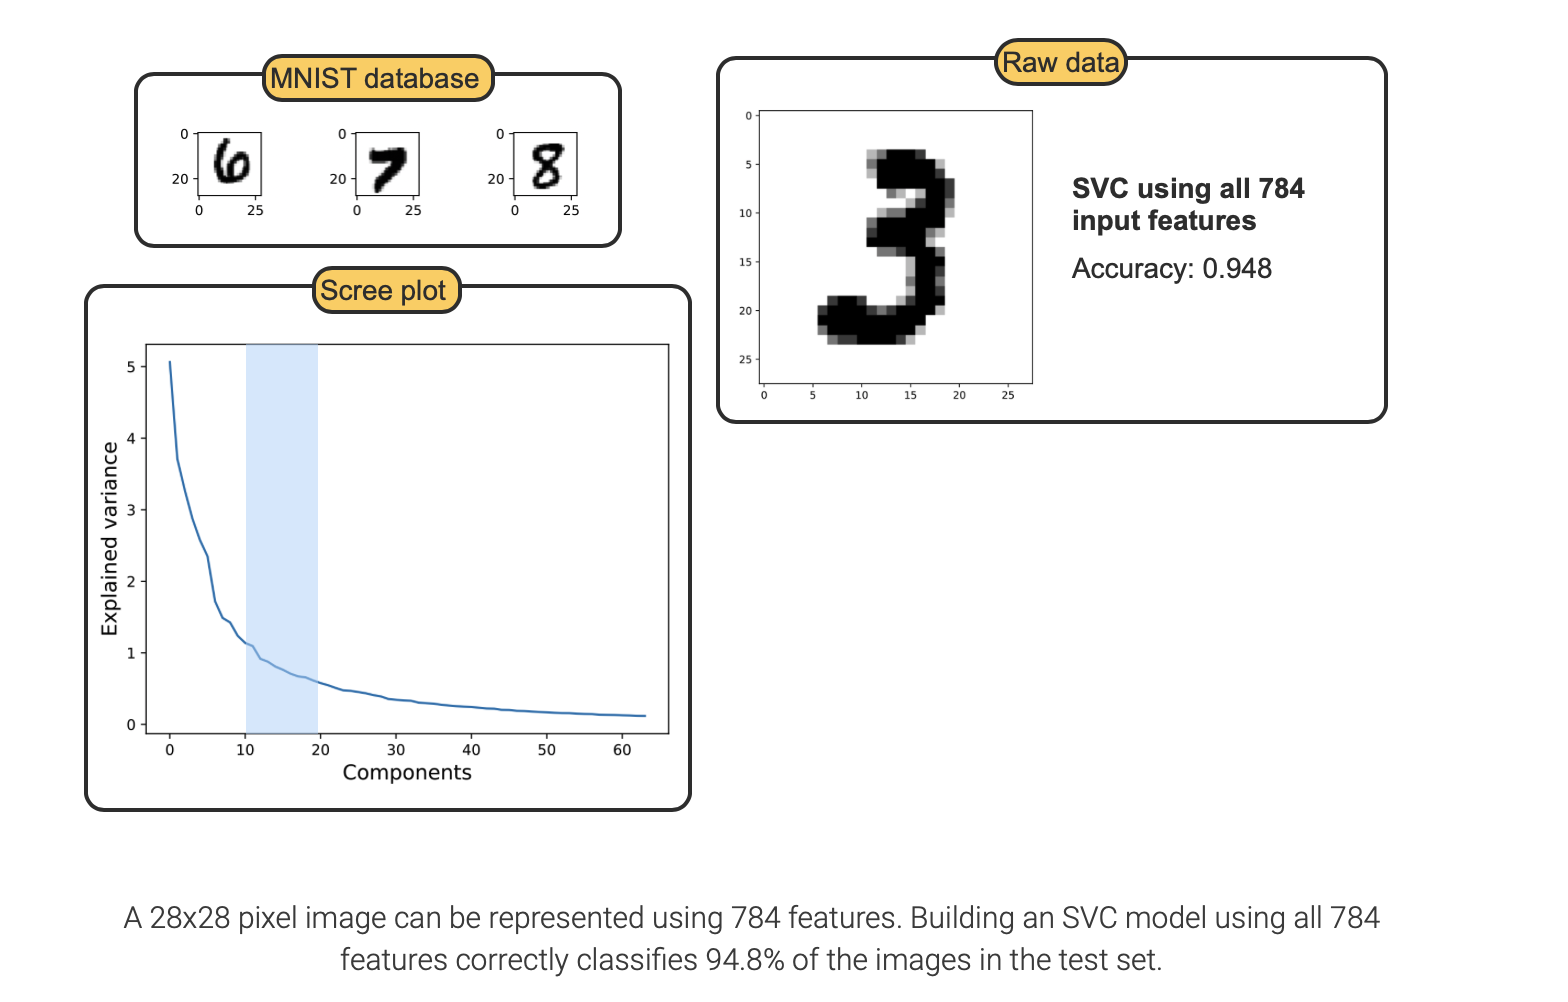
\includegraphics[width=0.8\textwidth]{imgs/DR_8.png}
    \end{figure}
\end{frame}

\begin{frame}
    \frametitle{Applying PCA to the MNIST digits dataset.}
    \begin{figure}[ht]
        \centering
        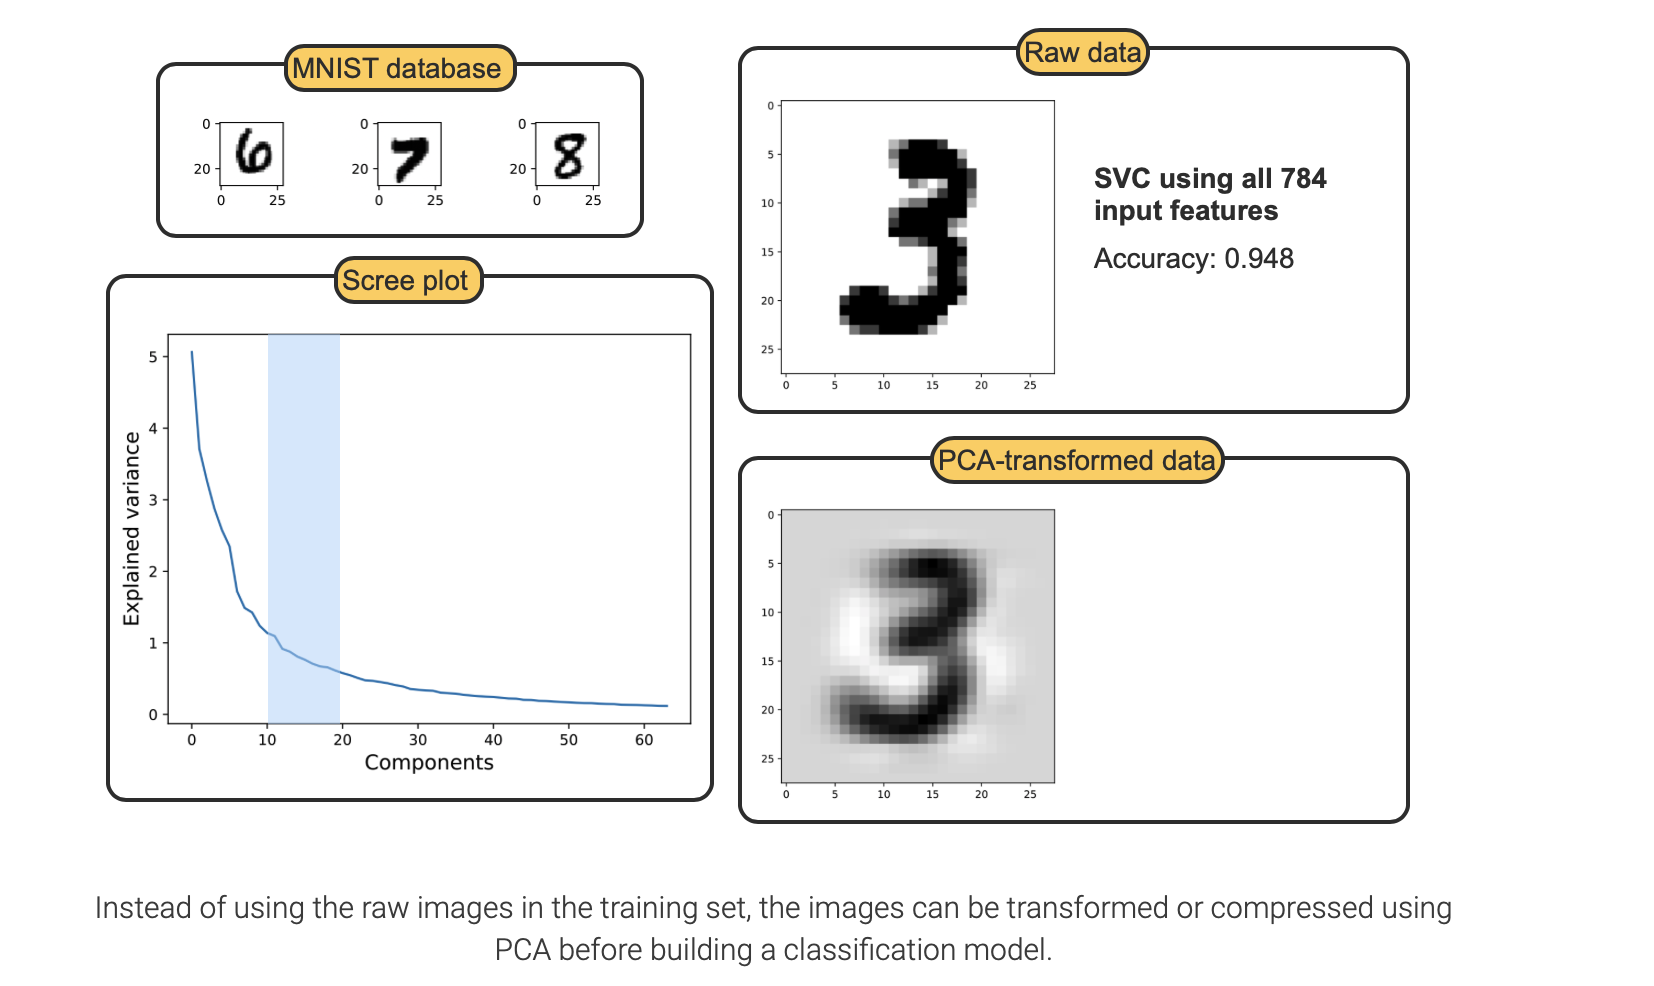
\includegraphics[width=0.8\textwidth]{imgs/DR_9.png}
    \end{figure}
\end{frame}

\begin{frame}
    \frametitle{Applying PCA to the MNIST digits dataset.}
    \begin{figure}[ht]
        \centering
        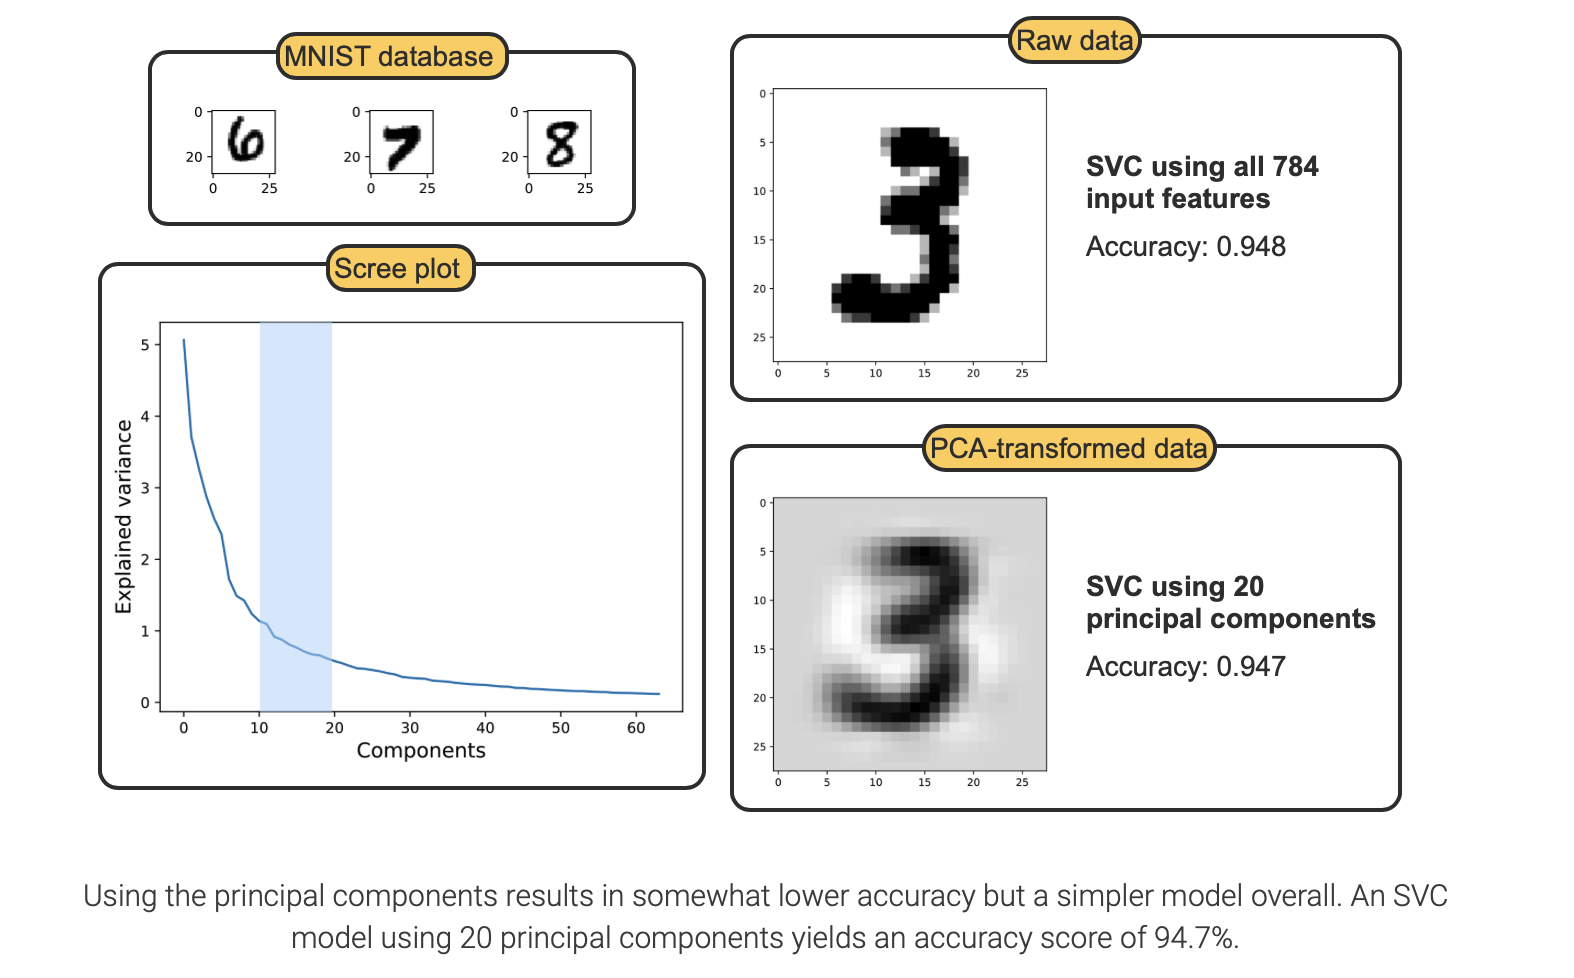
\includegraphics[width=0.8\textwidth]{imgs/DR_10.png}
    \end{figure}
\end{frame}
\end{document}